\documentclass{beamer}
\usepackage[utf8]{inputenc}
\usepackage{graphicx}
\usepackage{amsmath}
\usepackage{listings}
\usepackage{xcolor}

\title{ACO-TSP Paralelo em CPUs}
\author{Douglas Sousa Jorge\\Isaac Brasil Oliveira}
\date{}

\lstset{
  language=C,
  basicstyle=\footnotesize,
  numbers=left,
  numberstyle=\tiny\color{gray},
  stepnumber=1,
  numbersep=5pt,
  backgroundcolor=\color{white},
  showspaces=false,
  showstringspaces=false,
  showtabs=false,
  frame=single,
  rulecolor=\color{black},
  tabsize=2,
  captionpos=b,
  breaklines=true,
  breakatwhitespace=false,
  keywordstyle=\color{blue},
  commentstyle=\color{green},
  stringstyle=\color{red},
  escapeinside={\%*}{*)},
  morekeywords={*,...}
}

\begin{document}

\frame{\titlepage}

\begin{frame}
\frametitle{Problema}
\begin{itemize}
    \item O problema de otimização do Caixeiro Viajante (TSP) é um problema clássico de otimização combinatória.
    \item Objetivo: Encontrar o caminho mais curto que visita todas as cidades exatamente uma vez e retorna à cidade de origem.
    \item O desafio: Reduzir o tempo de execução ao resolver o TSP com algoritmos eficientes.
\end{itemize}
\end{frame}

\begin{frame}
\frametitle{Solução}
\begin{itemize}
    \item Utilização do Algoritmo de Otimização por Colônia de Formigas (ACO) para resolver o TSP.
    \item Implementação de duas versões:
    \begin{itemize}
        \item \textbf{Sequencial}: Algoritmo ACO executado de forma linear.
        \item \textbf{Paralelo}: Algoritmo ACO utilizando threads para paralelizar a construção das soluções.
    \end{itemize}
    \item Baseado nas metodologias descritas no paper original, adaptadas para execução em C\#.
\end{itemize}
\end{frame}

\begin{frame}
\frametitle{Metodologia}
\begin{itemize}
    \item \textbf{Experimentos}:
    \begin{itemize}
        \item Executar ambos os algoritmos (sequencial e paralelo) com diferentes números de iterações (1000, 5000, 10000, 50000, 100000).
        \item Medir o tempo de execução para cada caso.
        \item Comparar os resultados em termos de tempo de execução.
    \end{itemize}
    \item \textbf{Ferramentas}:
    \begin{itemize}
        \item C\# para implementação dos algoritmos.
        \item Bibliotecas: Parallel LINQ para paralelismo, System.IO para manipulação de arquivos.
    \end{itemize}
    \item \textbf{Paralelo com o paper original}:
    \begin{itemize}
        \item A implementação paralela segue a ideia do paper original, onde cada formiga é executada em uma thread separada.
    \end{itemize}
\end{itemize}
\end{frame}

\begin{frame}
\frametitle{Código Sequencial: Construção da Solução}
\begin{itemize}
    \item A construção da solução é feita com base nas probabilidades calculadas a partir dos feromônios e das heurísticas.
    \item As formigas escolhem a próxima cidade a ser visitada com base nessas probabilidades.
\end{itemize}
\begin{lstlisting}
int[] ConstruirSolucao(double[,] feromonios, double[,] heuristicas, int numCidades) {
    var tour = new int[numCidades];
    var visitadas = new bool[numCidades];
    var cidadeInicial = random.Next(numCidades);
    tour[0] = cidadeInicial;
    visitadas[cidadeInicial] = true;
    ...
    for (var i = 1; i < numCidades; i++) {
        ...
        probabilidades[j] = Math.Pow(feromonios[cidadeAtual, j], alpha) * Math.Pow(heuristicas[cidadeAtual, j], beta);
        ...
        tour[i] = proximaCidade;
        visitadas[proximaCidade] = true;
    }
    return tour;
}
\end{lstlisting}
\end{frame}

\begin{frame}
\frametitle{Código Sequencial: Atualização dos Feromônios}
\begin{itemize}
    \item Os feromônios são atualizados com base nas soluções encontradas pelas formigas.
\end{itemize}
\begin{lstlisting}
double[,] AtualizarFeromonios(int[][] tours, double[,] distancias, double[,] feromonios, double rho) {
    var deltaFeromonios = new double[numCidades, numCidades];
    foreach (var tour in tours) {
        for (var i = 0; i < tour.Length - 1; i++) {
            deltaFeromonios[tour[i], tour[i + 1]] += 1.0 / distancias[tour[i], tour[i + 1]];
        }
        deltaFeromonios[tour[^1], tour[0]] += 1.0 / distancias[tour[^1], tour[0]];
    }
    for (var i = 0; i < numCidades; i++) {
        for (var j = 0; j < numCidades; j++) {
            feromonios[i, j] = (1 - rho) * feromonios[i, j] + deltaFeromonios[i, j];
        }
    }
    return feromonios;
}
\end{lstlisting}
\end{frame}

\begin{frame}
\frametitle{Código Sequencial: Função Principal}
\begin{itemize}
    \item A função principal executa o algoritmo por um número especificado de iterações.
    \item Em cada iteração, as soluções são construídas e os feromônios são atualizados.
\end{itemize}
\begin{lstlisting}
void Aco(double[,] distancias, double[,] feromonios, double[,] heuristicas, int numCidades, int numFormigas, int numIteracoes) {
    for (var iteracao = 0; iteracao < numIteracoes; iteracao++) {
        var tours = new int[numFormigas][];
        for (var i = 0; i < numFormigas; i++) {
            tours[i] = ConstruirSolucao(feromonios, heuristicas, numCidades);
        }
        feromonios = AtualizarFeromonios(tours, distancias, feromonios, rho);
        Console.WriteLine($"Iteração {iteracao + 1}/{numIteracoes} concluída.");
    }
}
\end{lstlisting}
\end{frame}

\begin{frame}
\frametitle{Código Paralelo: Construção da Solução em Paralelo}
\begin{itemize}
    \item Utilização de \texttt{Parallel.For} para paralelizar a construção das soluções.
\end{itemize}
\begin{lstlisting}
Action<double[,], double[,], double[,], int, int, int> acoThread =
(distancias, feromonios, heuristicas, numCidades, numFormigas, numIteracoes) => {
    for (var iteracao = 0; iteracao < numIteracoes; iteracao++) {
        var tours = new int[numFormigas][];
        Parallel.For(0, numFormigas, i => {
            tours[i] = construirSolucao(feromonios, heuristicas, numCidades);
        });
        feromonios = atualizarFeromonios(tours, distancias, feromonios, rho);
        Console.WriteLine($"Iteração {iteracao + 1}/{numIteracoes} concluída.");
    }
};
\end{lstlisting}
\end{frame}

\begin{frame}
\frametitle{Resultados}
\begin{itemize}
    \item Tempos de execução foram registrados para diferentes números de iterações.
    \item Gráficos de comparação de tempo de execução e speedup foram gerados.
\end{itemize}
\end{frame}

\begin{frame}
\frametitle{Comparação do Tempo de Execução}
\begin{figure}[H]
    \centering
    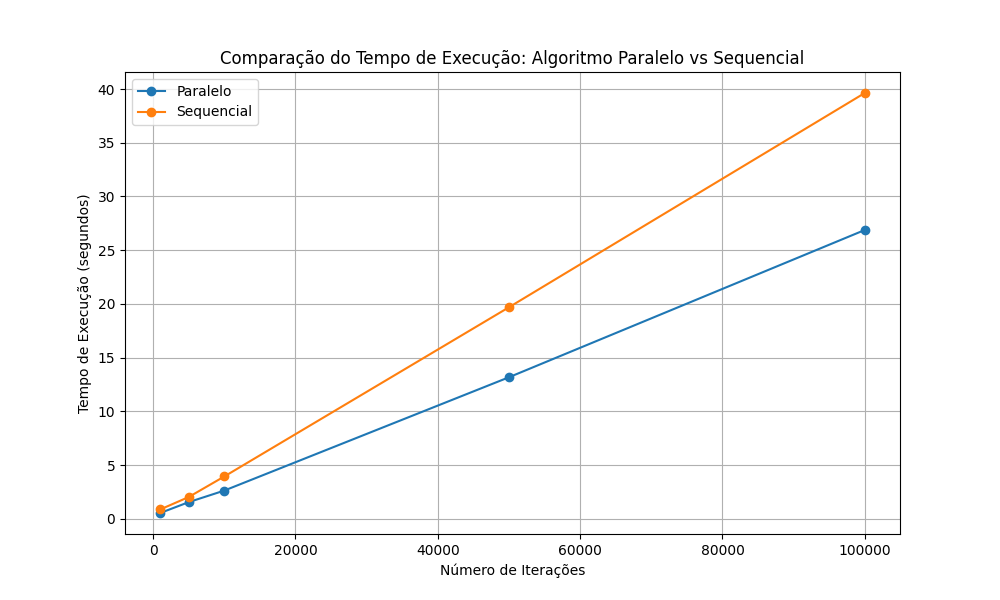
\includegraphics[width=0.8\linewidth]{comparacao_tempo_execucao.png}
    \caption{Comparação do Tempo de Execução: Algoritmo Paralelo vs Sequencial}
\end{figure}
\end{frame}

\begin{frame}
\frametitle{Speedup}
\begin{figure}[H]
    \centering
    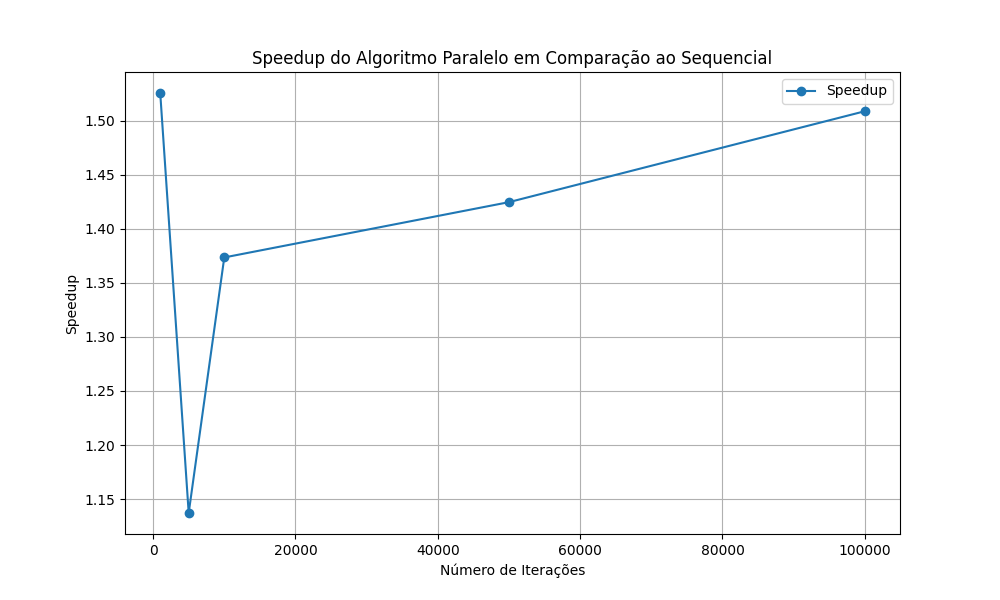
\includegraphics[width=0.8\linewidth]{speedup.png}
    \caption{Speedup do Algoritmo Paralelo em Comparação ao Sequencial}
\end{figure}
\end{frame}

\begin{frame}
\frametitle{Conclusão}
\begin{itemize}
    \item A implementação paralela do ACO mostra um speedup significativo em relação à versão sequencial.
    \item A eficiência do algoritmo paralelo aumenta com o número de iterações.
    \item O uso de técnicas de paralelismo pode melhorar significativamente o desempenho de algoritmos de otimização.
\end{itemize}
\end{frame}

\end{document}
